\documentclass[11pt, a4paper]{report}
\usepackage[utf8]{inputenc}
\usepackage[T1]{fontenc}
\usepackage{amsmath,amssymb,amsfonts,amsthm,mathtools}
\usepackage{geometry}
\geometry{a4paper, margin=0.8in, headheight=24pt, headsep=12pt}
\usepackage{lmodern}

\usepackage{xcolor}
\definecolor{primaryblue}{RGB}{13, 71, 161}    % Deep Blue #0D47A1
\definecolor{secondaryblue}{RGB}{25, 118, 210} % Medium Blue #1976D2
\definecolor{accentred}{RGB}{198, 40, 40}     % Dark Red #C62828
\definecolor{accentgreen}{RGB}{46, 125, 50}    % Dark Green #2E7D32
\definecolor{bglight}{RGB}{248, 249, 250}     % Soft Gray
\definecolor{bordergrey}{RGB}{207, 216, 220}  % Border Gray
\definecolor{darkslate}{RGB}{38, 50, 56}      % Slate

\usepackage{tcolorbox}

% Custom Callout Boxes
\newtcolorbox{defbox}[1][Definition]{%
  colback=primaryblue!5!white,
  colframe=primaryblue,
  fonttitle=\bfseries\color{white},
  title={Definition: #1},
  arc=4pt,
  boxrule=1.5pt,
  before skip=8pt,
  after skip=8pt
}

\newtcolorbox{theorembox}[1]{%
  colback=secondaryblue!5!white,
  colframe=secondaryblue,
  fonttitle=\bfseries\color{white},
  title={Theorem / Law: #1},
  arc=4pt,
  boxrule=1.5pt,
  before skip=8pt,
  after skip=8pt
}

\newtcolorbox{proofbox}[1]{%
  colback=white,
  colframe=accentgreen,
  fonttitle=\bfseries\color{white},
  title={Rigorous Proof / Derivation: #1},
  arc=4pt,
  boxrule=1.2pt,
  before skip=8pt,
  after skip=8pt
}

\newtcolorbox{keybox}[1][Key Concept]{%
  colback=accentred!5!white,
  colframe=accentred,
  fonttitle=\bfseries\color{white},
  title={#1},
  arc=4pt,
  boxrule=1.5pt,
  before skip=8pt,
  after skip=8pt
}

\usepackage{tikz}
\usetikzlibrary{arrows.meta, positioning, calc, angles, quotes, patterns, 3d, decorations.pathmorphing}

\usepackage{enumitem}
\usepackage{fancyhdr}
\pagestyle{fancy}
\fancyhf{}
\fancyhead[L]{\parbox[b]{0.65\textwidth}{\raggedright\small\color{darkslate}\nouppercase{\leftmark}}}
\fancyhead[R]{\small\color{primaryblue}\bfseries MTB 202 | sciqb.com}
\fancyfoot[L]{\sffamily\color{gray}\small Notes by Aryan (sciqb.com)}
\fancyfoot[C]{\thepage}
\fancyfoot[R]{\sffamily\color{secondaryblue}\small\bfseries\href{https://sciqb.com}{sciqb.com}}
\renewcommand{\headrulewidth}{0.5pt}

\fancypagestyle{plain}{%
  \fancyhf{}%
  \fancyfoot[L]{\sffamily\color{gray}\small Notes by Aryan (sciqb.com)}%
  \fancyfoot[C]{\thepage}%
  \fancyfoot[R]{\sffamily\color{secondaryblue}\small\bfseries\href{https://sciqb.com}{sciqb.com}}%
  \renewcommand{\headrulewidth}{0pt}%
}

\usepackage{hyperref}
\hypersetup{
    colorlinks=true,
    linkcolor=secondaryblue,
    citecolor=accentgreen,
    urlcolor=primaryblue,
    pdftitle={Complete Mechanics Proofs Manual - MTB 202},
    pdfauthor={Aryan (sciqb.com)}
}

\title{
    \vspace{-1.5cm}
    {\Huge\bfseries\color{primaryblue} CLASSICAL MECHANICS: MASTER PROOFS MANUAL}\\[0.4cm]
    {\Large\color{secondaryblue} Complete 42-Theorem Rigorous Derivation \& Diagram Handbook}\\[0.3cm]
    {\large\color{accentred}\bfseries Official Publication of \href{https://sciqb.com}{sciqb.com}}\\[0.5cm]
    \rule{0.8\textwidth}{1.5pt}
}
\author{
    \textbf{Aryan Maurya} \\
    Department of Mathematics, Institute of Science \\
    Banaras Hindu University (BHU) \\[1em]
    \small Complete Standalone Solution Manual with TikZ Diagrams for Every Proof (\href{https://sciqb.com}{sciqb.com})
}
\date{\today}

\begin{document}

\maketitle

\tableofcontents
\newpage

% ==============================================================================
% UNIT I: LAWS OF VECTORS IN 2D & SYSTEM OF COPLANAR FORCES
% ==============================================================================
\chapter{Laws of Vectors in 2D \& System of Coplanar Forces}

\section{Parallelogram Law of Forces}

\begin{theorembox}{Proof 1: Parallelogram Law of Forces}
If two coplanar forces $\mathbf{P}$ and $\mathbf{Q}$ acting simultaneously on a particle at point $O$ at angle $\alpha$ are represented in magnitude and direction by two adjacent sides of a parallelogram, their resultant $\mathbf{R}$ is represented in magnitude and direction by the diagonal passing through $O$:
\begin{equation}
R = \sqrt{P^2 + Q^2 + 2PQ\cos\alpha}, \qquad \tan\theta = \frac{Q\sin\alpha}{P + Q\cos\alpha}
\end{equation}
\end{theorembox}

\begin{proofbox}{Derivation of Parallelogram Law}
Let $OA$ represent force $P$ along $X$-axis and $OB$ represent force $Q$ at angle $\alpha$ to $OA$. Complete parallelogram $OACB$. Draw perpendicular $CD$ onto $OA$ produced.

\begin{center}
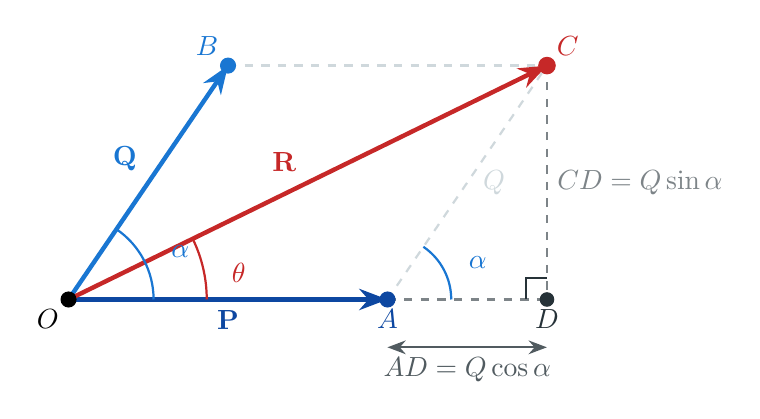
\begin{tikzpicture}[scale=1.35, >=Stealth]
    \coordinate (O) at (0,0);
    \coordinate (A) at (3.0,0);
    \coordinate (B) at (1.5, 2.2);
    \coordinate (C) at (4.5, 2.2);
    \coordinate (D) at (4.5, 0);

    \draw[dashed, darkslate!60, thick] (A) -- (D);
    \draw[dashed, darkslate!60, thick] (C) -- (D) node[midway, right] {$CD = Q\sin\alpha$};
    \draw[thick, darkslate] (4.3,0) -- (4.3, 0.2) -- (4.5, 0.2);

    \draw[thick, bordergrey, dashed] (B) -- (C);
    \draw[thick, bordergrey, dashed] (A) -- (C) node[midway, right=2pt] {$Q$};

    \draw[ultra thick, ->, primaryblue] (O) -- (A) node[midway, below] {$\mathbf{P}$};
    \draw[ultra thick, ->, secondaryblue] (O) -- (B) node[midway, above left] {$\mathbf{Q}$};
    \draw[ultra thick, ->, accentred] (O) -- (C) node[midway, above left, font=\bfseries] {$\mathbf{R}$};

    \filldraw[black] (O) circle (2pt) node[below left] {$O$};
    \filldraw[primaryblue] (A) circle (2pt) node[below] {$A$};
    \filldraw[secondaryblue] (B) circle (2pt) node[above left] {$B$};
    \filldraw[accentred] (C) circle (2.2pt) node[above right] {$C$};
    \filldraw[darkslate] (D) circle (1.8pt) node[below] {$D$};

    \draw[thick, secondaryblue] (0.8,0) arc (0:55.7:0.8);
    \node[secondaryblue] at (1.05, 0.45) {$\alpha$};
    \draw[thick, accentred] (1.3,0) arc (0:26.1:1.3);
    \node[accentred] at (1.6, 0.25) {$\theta$};
    \draw[thick, secondaryblue] (3.6,0) arc (0:55.7:0.6);
    \node[secondaryblue] at (3.85, 0.35) {$\alpha$};

    \draw[thick, <->, darkslate!80] (3.0, -0.45) -- (4.5, -0.45) node[midway, below] {$AD = Q\cos\alpha$};
\end{tikzpicture}
\end{center}

In right-angled triangle $\triangle ADC$: $AD = Q \cos\alpha, CD = Q \sin\alpha$.
In right-angled triangle $\triangle ODC$:
\[
OC^2 = OD^2 + CD^2 = (OA + AD)^2 + CD^2 = (P + Q\cos\alpha)^2 + (Q\sin\alpha)^2
\]
\[
R^2 = P^2 + 2PQ\cos\alpha + Q^2(\cos^2\alpha + \sin^2\alpha) = P^2 + Q^2 + 2PQ\cos\alpha \implies R = \sqrt{P^2 + Q^2 + 2PQ\cos\alpha}
\]
\[
\tan\theta = \frac{CD}{OD} = \frac{Q\sin\alpha}{P + Q\cos\alpha}
\]
\end{proofbox}

\section{Lami's Theorem}

\begin{theorembox}{Proof 2: Lami's Theorem}
If three coplanar concurrent forces $\mathbf{P}, \mathbf{Q}, \mathbf{R}$ acting at a point $O$ are in static equilibrium, each force is proportional to the sine of the angle between the other two forces:
\begin{equation}
\frac{P}{\sin\alpha} = \frac{Q}{\sin\beta} = \frac{R}{\sin\gamma}
\end{equation}
\end{theorembox}

\begin{proofbox}{Derivation of Lami's Theorem}
\begin{center}
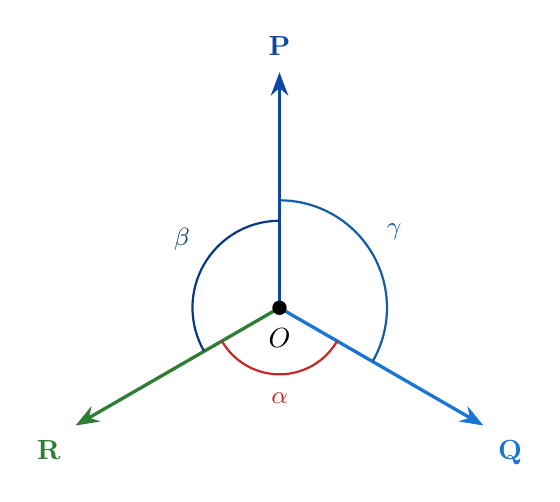
\begin{tikzpicture}[scale=1.3, >=Stealth]
    \coordinate (O) at (0,0);
    \coordinate (P) at (90:2.3);
    \coordinate (Q) at (-30:2.3);
    \coordinate (R) at (210:2.3);

    \draw[very thick, ->, color=primaryblue] (O) -- (P) node[above=2pt, font=\bfseries] {$\mathbf{P}$};
    \draw[very thick, ->, color=secondaryblue] (O) -- (Q) node[below right=2pt, font=\bfseries] {$\mathbf{Q}$};
    \draw[very thick, ->, color=accentgreen] (O) -- (R) node[below left=2pt, font=\bfseries] {$\mathbf{R}$};

    \fill (O) circle (2pt) node[below=4pt] {$O$};

    \draw[thick, color=accentred] (-30:0.65) arc (-30:-150:0.65) node[midway, below=3pt, font=\small\bfseries] {$\alpha$};
    \draw[thick, color=primaryblue!80!black] (90:0.85) arc (90:210:0.85) node[midway, above left=2pt, font=\small\bfseries] {$\beta$};
    \draw[thick, color=secondaryblue!80!black] (90:1.05) arc (90:-30:1.05) node[midway, above right=2pt, font=\small\bfseries] {$\gamma$};
\end{tikzpicture}
\end{center}

Since forces $\mathbf{P}, \mathbf{Q}, \mathbf{R}$ are in static equilibrium:
\[
\mathbf{P} + \mathbf{Q} + \mathbf{R} = \mathbf{0} \implies \mathbf{P} + \mathbf{Q} = -\mathbf{R}
\]
Taking vector cross product with $\mathbf{P}$:
\[
\mathbf{P} \times (\mathbf{P} + \mathbf{Q} + \mathbf{R}) = \mathbf{0} \implies \mathbf{P} \times \mathbf{Q} = \mathbf{R} \times \mathbf{P}
\]
Similarly, taking vector cross product with $\mathbf{Q}$:
\[
\mathbf{Q} \times \mathbf{R} = \mathbf{P} \times \mathbf{Q}
\]
Evaluating vector magnitudes:
\[
P Q \sin(180^\circ - \gamma) = Q R \sin(180^\circ - \alpha) = R P \sin(180^\circ - \beta)
\]
Dividing by $P Q R$:
\[
\frac{\sin\gamma}{R} = \frac{\sin\alpha}{P} = \frac{\sin\beta}{Q} \implies \frac{P}{\sin\alpha} = \frac{Q}{\sin\beta} = \frac{R}{\sin\gamma}
\]
\end{proofbox}

\section{System of Parallel Forces}

\begin{theorembox}{Proof 3 \& 4: Resultant of Like and Unlike Parallel Forces}
1. \textbf{Like Parallel Forces $P$ and $Q$}: Resultant $R = P + Q$ acting parallel to $P$ and $Q$ at internal point $C$ ($P \cdot AC = Q \cdot BC$).
2. \textbf{Unlike Parallel Forces $P > Q$}: Resultant $R = P - Q$ acting parallel to $P$ at external point $C$ ($P \cdot AC = Q \cdot BC$).
\end{theorembox}

\begin{proofbox}{Derivation of Parallel Forces Resultants}
\begin{center}
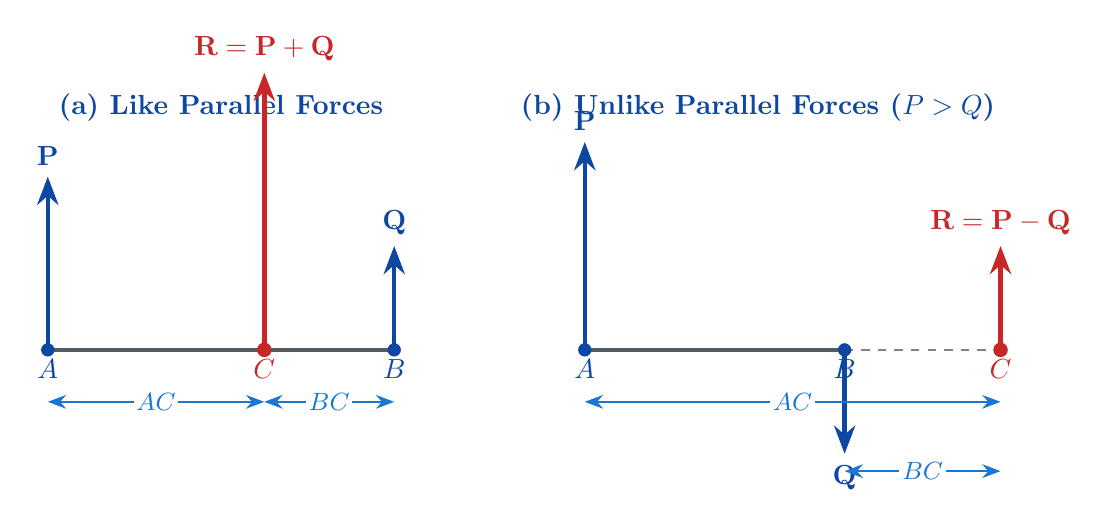
\begin{tikzpicture}[scale=1.1, >=Stealth]
    \begin{scope}[shift={(0,0)}]
        \node[font=\bfseries\color{primaryblue}] at (2.0, 2.8) {(a) Like Parallel Forces};
        \draw[ultra thick, darkslate!80] (0,0) -- (4,0);
        \filldraw[primaryblue] (0,0) circle (2pt) node[below] {$A$};
        \filldraw[primaryblue] (4,0) circle (2pt) node[below] {$B$};
        \filldraw[accentred] (2.5,0) circle (2.2pt) node[below] {$C$};
        \draw[ultra thick, ->, primaryblue] (0,0) -- (0, 2.0) node[above] {$\mathbf{P}$};
        \draw[ultra thick, ->, primaryblue] (4,0) -- (4, 1.2) node[above] {$\mathbf{Q}$};
        \draw[ultra thick, ->, accentred] (2.5,0) -- (2.5, 3.2) node[above] {$\mathbf{R} = \mathbf{P} + \mathbf{Q}$};
        \draw[thick, <->, secondaryblue] (0, -0.6) -- (2.5, -0.6) node[midway, fill=white, inner sep=1pt, font=\small] {$AC$};
        \draw[thick, <->, secondaryblue] (2.5, -0.6) -- (4.0, -0.6) node[midway, fill=white, inner sep=1pt, font=\small] {$BC$};
    \end{scope}

    \begin{scope}[shift={(6.2,0)}]
        \node[font=\bfseries\color{primaryblue}] at (2.0, 2.8) {(b) Unlike Parallel Forces ($P > Q$)};
        \draw[ultra thick, darkslate!80] (0,0) -- (3,0);
        \draw[dashed, darkslate!60, thick] (3,0) -- (4.8,0);
        \filldraw[primaryblue] (0,0) circle (2pt) node[below] {$A$};
        \filldraw[primaryblue] (3,0) circle (2pt) node[below] {$B$};
        \filldraw[accentred] (4.8,0) circle (2.2pt) node[below] {$C$};
        \draw[ultra thick, ->, primaryblue] (0,0) -- (0, 2.4) node[above] {$\mathbf{P}$};
        \draw[ultra thick, ->, primaryblue] (3,0) -- (3, -1.2) node[below] {$\mathbf{Q}$};
        \draw[ultra thick, ->, accentred] (4.8,0) -- (4.8, 1.2) node[above] {$\mathbf{R} = \mathbf{P} - \mathbf{Q}$};
        \draw[thick, <->, secondaryblue] (0, -0.6) -- (4.8, -0.6) node[midway, fill=white, inner sep=1pt, font=\small] {$AC$};
        \draw[thick, <->, secondaryblue] (3.0, -1.4) -- (4.8, -1.4) node[midway, fill=white, inner sep=1pt, font=\small] {$BC$};
    \end{scope}
\end{tikzpicture}
\end{center}

Taking moments about base point $A$:
\[
R \cdot AC = Q \cdot AB \implies (P \pm Q) \cdot AC = Q \cdot (AC \pm BC) \implies P \cdot AC = Q \cdot BC \implies \frac{AC}{BC} = \frac{Q}{P}
\]
\end{proofbox}

\begin{theorembox}{Proof 5: Center of Parallel Forces}
The position vector $\mathbf{r}_C$ of the center of a system of parallel forces $\mathbf{F}_i = F_i \hat{u}$ acting at points $\mathbf{r}_i$ is independent of the direction $\hat{u}$:
\begin{equation}
\mathbf{r}_C = \frac{\sum_{i=1}^n F_i \mathbf{r}_i}{\sum_{i=1}^n F_i}
\end{equation}
\end{theorembox}

\begin{proofbox}{Derivation of Center of Parallel Forces}
\begin{center}
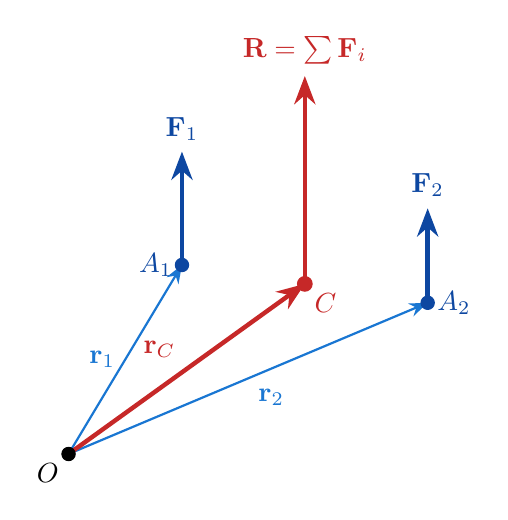
\begin{tikzpicture}[scale=1.2, >=Stealth]
    \coordinate (O) at (0,0);
    \coordinate (A1) at (1.2, 2.0);
    \coordinate (A2) at (3.8, 1.6);
    \coordinate (C) at (2.5, 1.8);

    \draw[thick, ->, secondaryblue] (O) -- (A1) node[midway, left] {$\mathbf{r}_1$};
    \draw[thick, ->, secondaryblue] (O) -- (A2) node[midway, below right] {$\mathbf{r}_2$};
    \draw[ultra thick, ->, accentred] (O) -- (C) node[midway, above left] {$\mathbf{r}_C$};

    \draw[ultra thick, ->, primaryblue] (A1) -- ++(0, 1.2) node[above] {$\mathbf{F}_1$};
    \draw[ultra thick, ->, primaryblue] (A2) -- ++(0, 1.0) node[above] {$\mathbf{F}_2$};
    \draw[ultra thick, ->, accentred] (C) -- ++(0, 2.2) node[above] {$\mathbf{R} = \sum \mathbf{F}_i$};

    \filldraw[black] (O) circle (2pt) node[below left] {$O$};
    \filldraw[primaryblue] (A1) circle (2pt) node[left] {$A_1$};
    \filldraw[primaryblue] (A2) circle (2pt) node[right] {$A_2$};
    \filldraw[accentred] (C) circle (2.2pt) node[below right] {$C$};
\end{tikzpicture}
\end{center}

Total vector moment about origin $O$:
\[
\mathbf{G}_O = \sum_{i=1}^n (\mathbf{r}_i \times \mathbf{F}_i) = \sum_{i=1}^n (\mathbf{r}_i \times F_i \hat{u}) = \left( \sum_{i=1}^n F_i \mathbf{r}_i \right) \times \hat{u}
\]
Equating to moment of single resultant force $\mathbf{R} = (\sum F_i)\hat{u}$ acting at $\mathbf{r}_C$:
\[
\mathbf{r}_C \times \mathbf{R} = \mathbf{r}_C \times \left( \sum F_i \hat{u} \right) = \left( \mathbf{r}_C \sum F_i \right) \times \hat{u}
\]
Comparing coefficients yields $\mathbf{r}_C \sum F_i = \sum F_i \mathbf{r}_i \implies \mathbf{r}_C = \frac{\sum F_i \mathbf{r}_i}{\sum F_i}$.
\end{proofbox}

\section{Theory of Couples \& Moments}

\begin{theorembox}{Proof 6: Origin Invariance of Couple Moment}
The vector moment of a couple $(-\mathbf{P}, +\mathbf{P})$ acting at $A(\mathbf{r}_A)$ and $B(\mathbf{r}_B)$ is an invariant free vector independent of reference origin $O$:
\begin{equation}
\mathbf{G}_O = \mathbf{r}_{AB} \times \mathbf{P}
\end{equation}
\end{theorembox}

\begin{proofbox}{Derivation of Couple Moment Invariance}
\begin{center}
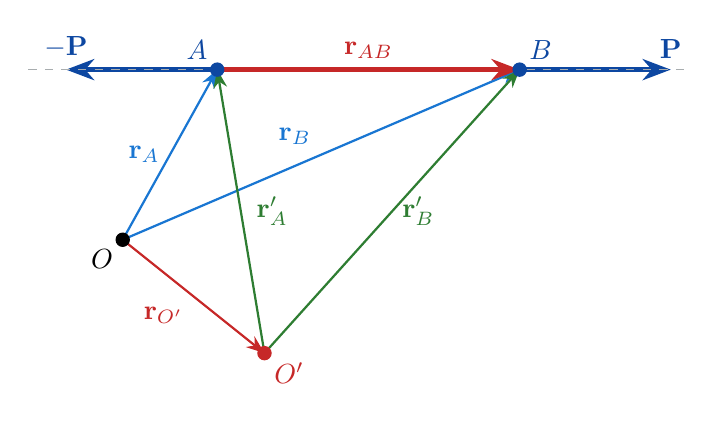
\begin{tikzpicture}[scale=1.2, >=Stealth]
    \coordinate (O) at (0,0);
    \coordinate (Oprime) at (1.5, -1.2);
    \coordinate (A) at (1.0, 1.8);
    \coordinate (B) at (4.2, 1.8);

    \draw[ultra thick, ->, primaryblue] (A) -- ($(A) + (-1.6, 0)$) node[above] {$-\mathbf{P}$};
    \draw[ultra thick, ->, primaryblue] (B) -- ($(B) + (1.6, 0)$) node[above] {$\mathbf{P}$};
    \draw[dashed, darkslate!40] (-1.0, 1.8) -- (6.0, 1.8);

    \draw[thick, ->, secondaryblue] (O) -- (A) node[midway, left] {$\mathbf{r}_A$};
    \draw[thick, ->, secondaryblue] (O) -- (B) node[midway, above left] {$\mathbf{r}_B$};
    \draw[thick, ->, accentgreen] (Oprime) -- (A) node[midway, right=2pt] {$\mathbf{r}'_A$};
    \draw[thick, ->, accentgreen] (Oprime) -- (B) node[midway, right] {$\mathbf{r}'_B$};
    \draw[thick, ->, accentred] (O) -- (Oprime) node[midway, below left] {$\mathbf{r}_{O'}$};
    \draw[ultra thick, ->, accentred] (A) -- (B) node[midway, above] {$\mathbf{r}_{AB}$};

    \filldraw[black] (O) circle (2pt) node[below left] {$O$};
    \filldraw[accentred] (Oprime) circle (2pt) node[below right] {$O'$};
    \filldraw[primaryblue] (A) circle (2pt) node[above left] {$A$};
    \filldraw[primaryblue] (B) circle (2pt) node[above right] {$B$};
\end{tikzpicture}
\end{center}

Moment about origin $O$: $\mathbf{G}_O = \mathbf{r}_A \times (-\mathbf{P}) + \mathbf{r}_B \times \mathbf{P} = (\mathbf{r}_B - \mathbf{r}_A) \times \mathbf{P} = \mathbf{r}_{AB} \times \mathbf{P}$.\\
Moment about shifted origin $O'$ ($\mathbf{r}'_A = \mathbf{r}_A - \mathbf{r}_{O'}, \mathbf{r}'_B = \mathbf{r}_B - \mathbf{r}_{O'}$):
\[
\mathbf{G}_{O'} = (\mathbf{r}_A - \mathbf{r}_{O'}) \times (-\mathbf{P}) + (\mathbf{r}_B - \mathbf{r}_{O'}) \times \mathbf{P} = (\mathbf{r}_B - \mathbf{r}_A) \times \mathbf{P} = \mathbf{G}_O
\]
Thus, the moment of a couple is completely invariant under shift of origin.
\end{proofbox}

\begin{theorembox}{Proof 7: Varignon's Theorem of Moments}
The algebraic sum of vector moments of two coplanar forces $\mathbf{P}$ and $\mathbf{Q}$ about any point $O$ equals the moment of their resultant $\mathbf{R} = \mathbf{P} + \mathbf{Q}$ about $O$:
\begin{equation}
\mathbf{M}_O(\mathbf{R}) = \mathbf{M}_O(\mathbf{P}) + \mathbf{M}_O(\mathbf{Q})
\end{equation}
\end{theorembox}

\begin{proofbox}{Derivation of Varignon's Theorem}
\begin{center}
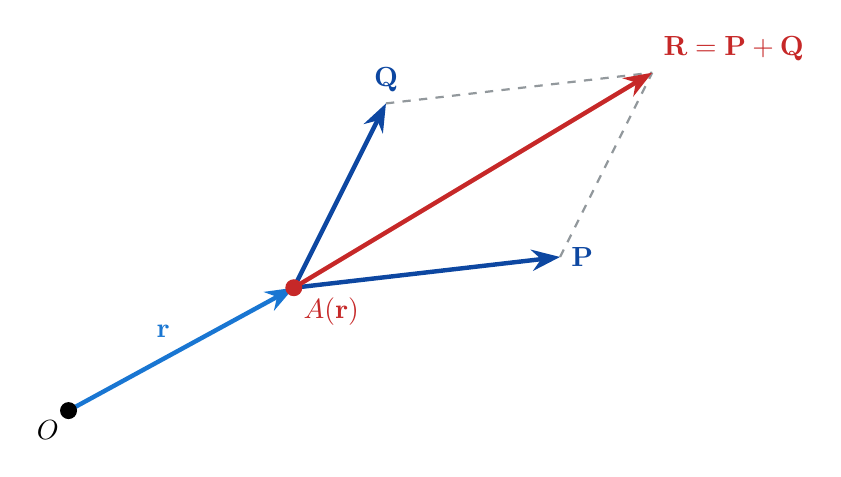
\begin{tikzpicture}[scale=1.3, >=Stealth]
    \coordinate (O) at (0, 0);
    \coordinate (A) at (2.2, 1.2);
    \coordinate (P) at ($(A) + (2.6, 0.3)$);
    \coordinate (Q) at ($(A) + (0.9, 1.8)$);
    \coordinate (R) at ($(A) + (3.5, 2.1)$);

    \draw[ultra thick, ->, secondaryblue] (O) -- (A) node[midway, above left] {$\mathbf{r}$};
    \draw[dashed, darkslate!50, thick] (P) -- (R);
    \draw[dashed, darkslate!50, thick] (Q) -- (R);
    \draw[ultra thick, ->, primaryblue] (A) -- (P) node[right] {$\mathbf{P}$};
    \draw[ultra thick, ->, primaryblue] (A) -- (Q) node[above] {$\mathbf{Q}$};
    \draw[ultra thick, ->, accentred] (A) -- (R) node[above right] {$\mathbf{R} = \mathbf{P} + \mathbf{Q}$};

    \filldraw[black] (O) circle (2.2pt) node[below left] {$O$};
    \filldraw[accentred] (A) circle (2.2pt) node[below right] {$A(\mathbf{r})$};
\end{tikzpicture}
\end{center}

Taking vector cross product of position vector $\mathbf{r}$ with resultant $\mathbf{R} = \mathbf{P} + \mathbf{Q}$:
\[
\mathbf{r} \times \mathbf{R} = \mathbf{r} \times (\mathbf{P} + \mathbf{Q}) = (\mathbf{r} \times \mathbf{P}) + (\mathbf{r} \times \mathbf{Q}) \implies \mathbf{M}_O(\mathbf{R}) = \mathbf{M}_O(\mathbf{P}) + \mathbf{M}_O(\mathbf{Q})
\]
\end{proofbox}

\section{Reduction of Coplanar System \& Line of Action}

\begin{theorembox}{Proof 8 \& 9: Reduction of Coplanar Forces and Line of Action}
1. \textbf{Reduction}: Any system of coplanar forces $(X_i, Y_i)$ acting at $(x_i, y_i)$ reduces at origin $O$ to a single force $(X, Y)$ and a couple $G = \sum (x_i Y_i - y_i X_i)$.
2. \textbf{Line of Action}: The equation of the line of action of resultant $R = \sqrt{X^2 + Y^2}$ is:
\begin{equation}
xY - yX = G
\end{equation}
\end{theorembox}

\begin{proofbox}{Derivation of Reduction and Line of Action}
\begin{center}
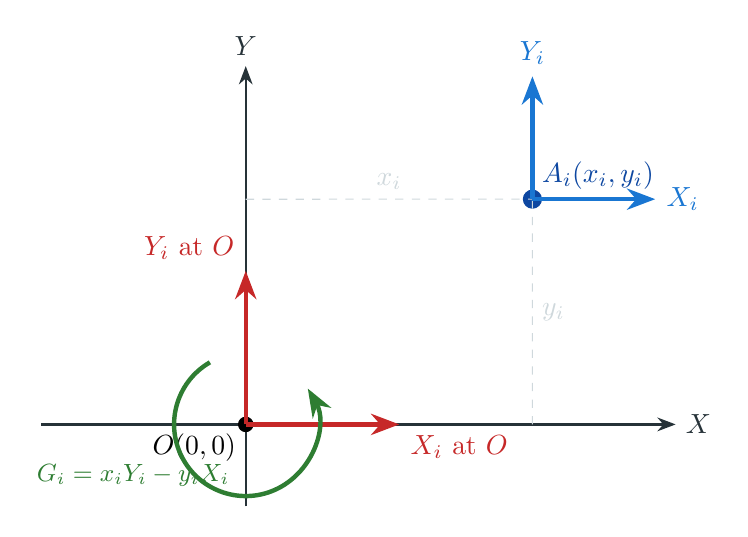
\begin{tikzpicture}[scale=1.3, >=Stealth]
    \draw[->, thick, darkslate] (-2.0, 0) -- (4.2, 0) node[right] {$X$};
    \draw[->, thick, darkslate] (0, -0.8) -- (0, 3.5) node[above] {$Y$};
    \filldraw[black] (0,0) circle (2pt) node[below left] {$O(0,0)$};

    \coordinate (A) at (2.8, 2.2);
    \filldraw[primaryblue] (A) circle (2.5pt) node[above right] {$A_i(x_i, y_i)$};
    \draw[dashed, bordergrey] (2.8,0) -- (A) node[midway, right] {$y_i$};
    \draw[dashed, bordergrey] (0,2.2) -- (A) node[midway, above] {$x_i$};

    \draw[ultra thick, ->, secondaryblue] (A) -- ($(A) + (1.2, 0)$) node[right] {$X_i$};
    \draw[ultra thick, ->, secondaryblue] (A) -- ($(A) + (0, 1.2)$) node[above] {$Y_i$};
    \draw[ultra thick, ->, accentred] (0,0) -- (1.5, 0) node[below right] {$X_i$ at $O$};
    \draw[ultra thick, ->, accentred] (0,0) -- (0, 1.5) node[above left] {$Y_i$ at $O$};

    \draw[ultra thick, ->, accentgreen] (120:0.7) arc (120:390:0.7);
    \node[accentgreen, font=\small] at (-1.1, -0.5) {$G_i = x_i Y_i - y_i X_i$};
\end{tikzpicture}
\end{center}

Transferring force $(X_i, Y_i)$ at $A_i(x_i, y_i)$ to origin $O$ introduces an equivalent force $(X_i, Y_i)$ at $O$ plus a couple moment $G_i = x_i Y_i - y_i X_i$. Summing over all forces yields $X = \sum X_i, Y = \sum Y_i, G = \sum (x_i Y_i - y_i X_i)$.

Shift base point from $O(0,0)$ to $O'(\xi, \eta)$. New couple moment $G' = G - \xi Y + \eta X$. For $O'(\xi, \eta)$ to lie on the line of action of resultant force $R$, couple moment must vanish ($G' = 0$):
\[
G - \xi Y + \eta X = 0 \implies \xi Y - \eta X = G \implies xY - yX = G
\]
\end{proofbox}

% ==============================================================================
% UNIT II: EQUILIBRIUM OF FORCES IN 2D & PRINCIPLE OF VIRTUAL WORK
% ==============================================================================
\chapter{Equilibrium of Forces in 2D \& Principle of Virtual Work}

\section{Analytical Conditions of Equilibrium}

\begin{theorembox}{Proof 10 \& 11: Conditions of Equilibrium \& 3-Point Moment Form}
1. \textbf{Standard Form}: Coplanar forces are in equilibrium if and only if $X = \sum X_i = 0, Y = \sum Y_i = 0, G = \sum M_O = 0$.
2. \textbf{Three-Point Form}: For non-collinear points $A, B, C$, equilibrium holds iff $M_A = 0, M_B = 0, M_C = 0$.
\end{theorembox}

\begin{proofbox}{Derivation of 2D Equilibrium Conditions}
\begin{center}
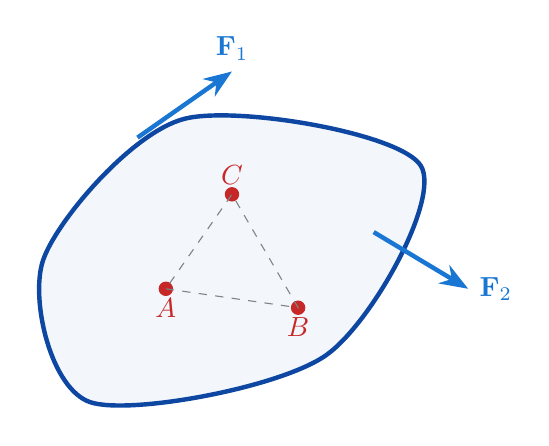
\begin{tikzpicture}[scale=1.2, >=Stealth]
    \draw[ultra thick, primaryblue, fill=primaryblue!5] plot [smooth cycle] 
        coordinates {(0,0) (2.5,0.5) (3.5,2.5) (1.0,3.0) (-0.5,1.5)};
    
    \filldraw[accentred] (0.8, 1.2) circle (2pt) node[below] {$A$};
    \filldraw[accentred] (2.2, 1.0) circle (2pt) node[below] {$B$};
    \filldraw[accentred] (1.5, 2.2) circle (2pt) node[above] {$C$};
    \draw[dashed, darkslate!60] (0.8, 1.2) -- (2.2, 1.0) -- (1.5, 2.2) -- cycle;
    
    \draw[ultra thick, ->, secondaryblue] (0.5, 2.8) -- (1.5, 3.5) node[above] {$\mathbf{F}_1$};
    \draw[ultra thick, ->, secondaryblue] (3.0, 1.8) -- (4.0, 1.2) node[right] {$\mathbf{F}_2$};
\end{tikzpicture}
\end{center}

Resultant force magnitude $R = \sqrt{X^2 + Y^2}$ and couple $G$. For complete equilibrium, no translational motion requires $R = 0 \implies X = 0, Y = 0$, and no rotational motion requires $G = 0$.\\
If $M_A = 0$, resultant $R$ must either be zero or pass through $A$. If $M_B = 0$, $R$ must pass through $B$. Thus line of action of $R$ is line $AB$. If $M_C = 0$ where $C$ is not on line $AB$, $R$ cannot pass through $C$ unless $R = 0$. Hence $R = 0$ and $G = 0$.
\end{proofbox}

\section{Principle of Virtual Work}

\begin{theorembox}{Proof 12: Principle of Virtual Work}
A coplanar system of rigid bodies is in static equilibrium if and only if the net virtual work performed by all active forces vanishes for every small arbitrary virtual displacement:
\begin{equation}
\sum \delta W = \sum_{i=1}^n (X_i \, \delta x_i + Y_i \, \delta y_i) = 0
\end{equation}
\end{theorembox}

\begin{proofbox}{Derivation of Virtual Work Principle}
\begin{center}
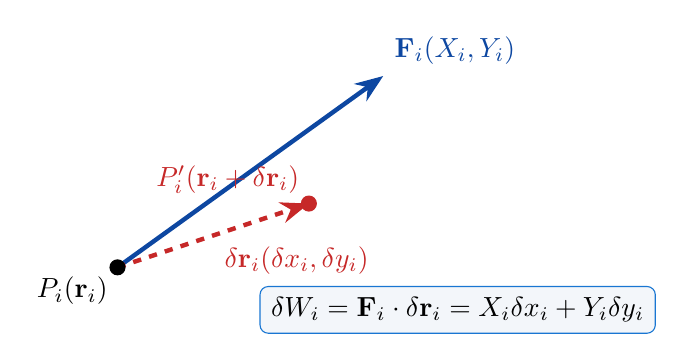
\begin{tikzpicture}[scale=1.35, >=Stealth]
    \coordinate (A) at (0, 0);
    \coordinate (Aprime) at (1.8, 0.6);
    \draw[ultra thick, ->, primaryblue] (A) -- (2.5, 1.8) node[above right] {$\mathbf{F}_i(X_i, Y_i)$};
    \draw[ultra thick, ->, accentred, dashed] (A) -- (Aprime) node[midway, below right] {$\delta\mathbf{r}_i(\delta x_i, \delta y_i)$};

    \filldraw[black] (A) circle (2pt) node[below left] {$P_i(\mathbf{r}_i)$};
    \filldraw[accentred] (Aprime) circle (2pt) node[above left] {$P'_i(\mathbf{r}_i + \delta\mathbf{r}_i)$};
    \node[draw=secondaryblue, fill=primaryblue!5, rounded corners=3pt, inner sep=4pt] at (3.2, -0.4) {$\delta W_i = \mathbf{F}_i \cdot \delta\mathbf{r}_i = X_i\delta x_i + Y_i\delta y_i$};
\end{tikzpicture}
\end{center}

For a particle $P_i$ at $(x_i, y_i)$ under force $\mathbf{F}_i(X_i, Y_i)$, giving a virtual displacement $\delta\mathbf{r}_i(\delta x_i, \delta y_i)$, virtual work is $\delta W_i = \mathbf{F}_i \cdot \delta\mathbf{r}_i = X_i \delta x_i + Y_i \delta y_i$. Summing over system: $\sum \delta W_i = \sum (X_i \delta x_i + Y_i \delta y_i)$. If in equilibrium, $\mathbf{F}_{\text{net}} = \mathbf{0} \implies \sum \delta W = 0$.
\end{proofbox}

\begin{theorembox}{Proof 13 \& 14: Constraint Forces and Active Work Expressions}
1. \textbf{Constraints}: Reactions at smooth surfaces, fixed hinges, inextensible strings, and rolling without slipping do **zero** net virtual work.
2. \textbf{Active Work}: Gravity $W$: $\delta W = -W \delta y_{cg}$; Elastic String $T$: $\delta W = -T \delta l$; Rod Thrust $S$: $\delta W = +S \delta x$.
\end{theorembox}

\begin{proofbox}{Derivation of Active Force Work Terms}
\begin{center}
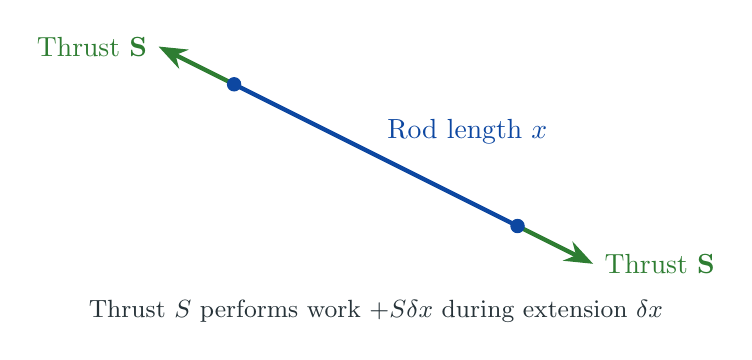
\begin{tikzpicture}[scale=1.2, >=Stealth]
    \draw[ultra thick, primaryblue] (0, 2.0) -- (3.0, 0.5) node[midway, above right] {Rod length $x$};
    \draw[ultra thick, ->, accentgreen] (0, 2.0) -- (-0.8, 2.4) node[left] {Thrust $\mathbf{S}$};
    \draw[ultra thick, ->, accentgreen] (3.0, 0.5) -- (3.8, 0.1) node[right] {Thrust $\mathbf{S}$};
    \filldraw[primaryblue] (0, 2.0) circle (2pt);
    \filldraw[primaryblue] (3.0, 0.5) circle (2pt);

    \node[font=\small\color{darkslate}] at (1.5, -0.4) {Thrust $S$ performs work $+S \delta x$ during extension $\delta x$};
\end{tikzpicture}
\end{center}

For gravity, potential energy is $V = W y_{cg} \implies \delta W = -\delta V = -W \delta y_{cg}$.\\
For a tension $T$ pulling two endpoints inwards separated by distance $l$, virtual work for extension $\delta l$ is $\delta W = -T \delta l$.\\
For thrust $S$ pushing endpoints outwards separated by length $x$, virtual work for extension $\delta x$ is $\delta W = +S \delta x$.
\end{proofbox}

\begin{theorembox}{Proof 15: Application of Hooke's Law}
Tension $T = \lambda \frac{l - a}{a}$ in elastic string of natural length $a$ stretched to $l$. Substituting into virtual work yields:
\begin{equation}
\delta W_{\text{elastic}} = -T \delta l = -\lambda \left(\frac{l - a}{a}\right) \delta l
\end{equation}
\end{theorembox}

\begin{proofbox}{Derivation of Hooke's Law Virtual Work}
\begin{center}

\begin{tikzpicture}[scale=1.2, >=Stealth]
    \draw[ultra thick, darkslate] (0,0) -- (1.5, 0) node[midway, above] {Natural $a$};
    \draw[ultra thick, primaryblue, decoration={aspect=0.4, segment length=5pt, amplitude=6pt}, decorate] (1.5, 0) -- (4.0, 0) node[midway, above=6pt] {Stretching $(l - a)$};
    \draw[ultra thick, ->, accentred] (4.0, 0) -- (2.8, 0) node[below] {Tension $T$};
    \filldraw[accentred] (4.0, 0) circle (2pt) node[right] {Endpoint};
\end{tikzpicture}
\end{center}

Hooke's Law states tension is proportional to extension per unit natural length: $T = \lambda \left(\frac{l-a}{a}\right)$.
Work done by tension during small extension $\delta l$ is $\delta W = -T \delta l = -\lambda \left(\frac{l-a}{a}\right) \delta l$.
\end{proofbox}

\section{Stability of Equilibrium}

\begin{theorembox}{Proof 16: Stability Criteria of Equilibrium}
For conservative system with potential energy $V(\theta)$: Equilibrium holds if $V'(\theta) = 0$.
1. **Stable**: $V''(\theta) > 0$ (PE is a minimum).
2. **Unstable**: $V''(\theta) < 0$ (PE is a maximum).
3. **Neutral**: $V''(\theta) = 0$.
\end{theorembox}

\begin{proofbox}{Derivation of Stability Criteria}
\begin{center}
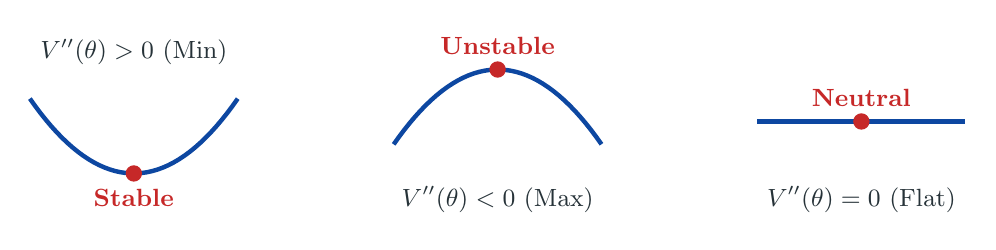
\begin{tikzpicture}[scale=1.1, >=Stealth]
    \begin{scope}[shift={(0,0)}]
        \draw[ultra thick, primaryblue, domain=-1.2:1.2, samples=40] plot (\x, {0.6*\x*\x});
        \filldraw[accentred] (0,0) circle (2.5pt) node[below=2pt, font=\small\bfseries] {Stable};
        \node[font=\small\color{darkslate}] at (0, 1.4) {$V''(\theta) > 0$ (Min)};
    \end{scope}
    \begin{scope}[shift={(4.2,0)}]
        \draw[ultra thick, primaryblue, domain=-1.2:1.2, samples=40] plot (\x, {1.2 - 0.6*\x*\x});
        \filldraw[accentred] (0,1.2) circle (2.5pt) node[above=2pt, font=\small\bfseries] {Unstable};
        \node[font=\small\color{darkslate}] at (0, -0.3) {$V''(\theta) < 0$ (Max)};
    \end{scope}
    \begin{scope}[shift={(8.4,0)}]
        \draw[ultra thick, primaryblue] (-1.2, 0.6) -- (1.2, 0.6);
        \filldraw[accentred] (0,0.6) circle (2.5pt) node[above=2pt, font=\small\bfseries] {Neutral};
        \node[font=\small\color{darkslate}] at (0, -0.3) {$V''(\theta) = 0$ (Flat)};
    \end{scope}
\end{tikzpicture}
\end{center}

Expanding $V(\theta)$ about equilibrium position $\theta_0$ using Taylor series ($\theta = \theta_0 + x$):
\[
V(\theta) = V(\theta_0) + x V'(\theta_0) + \frac{x^2}{2} V''(\theta_0) + \dots
\]
Since $V'(\theta_0) = 0$, $\Delta V = V(\theta) - V(\theta_0) \approx \frac{1}{2} x^2 V''(\theta_0)$. If $V''(\theta_0) > 0$, $\Delta V > 0$ (potential energy increases upon displacement), creating a restoring force towards $\theta_0$ (Stable). If $V''(\theta_0) < 0$, $\Delta V < 0$, creating a driving force away from $\theta_0$ (Unstable).
\end{proofbox}

% ==============================================================================
% UNIT III: KINEMATICS & DYNAMICS OF A PARTICLE IN 2D (SHM)
% ==============================================================================
\chapter{Kinematics \& Dynamics of a Particle in 2D (SHM)}

\section{Polar Coordinates Kinematics}

\begin{theorembox}{Proof 17 \& 18: Radial and Transverse Velocity and Acceleration}
1. \textbf{Velocity Components}: Radial $v_r = \dot{r}$, Transverse $v_\theta = r\dot{\theta}$.
2. \textbf{Acceleration Components}: Radial $a_r = \ddot{r} - r\dot{\theta}^2$, Transverse $a_\theta = \frac{1}{r}\frac{d}{dt}(r^2\dot{\theta}) = 2\dot{r}\dot{\theta} + r\ddot{\theta}$.
\end{theorembox}

\begin{proofbox}{Derivation of Polar Velocity and Acceleration}
\begin{center}
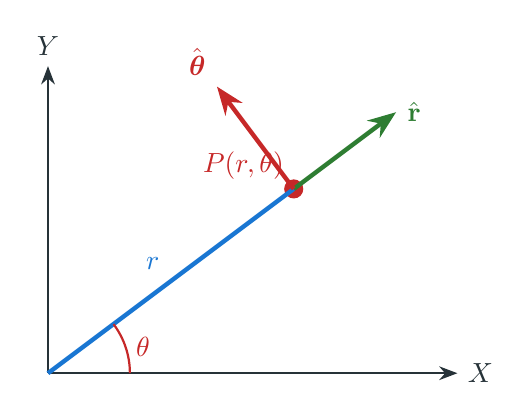
\begin{tikzpicture}[scale=1.3, >=Stealth]
    \draw[->, thick, darkslate] (0,0) -- (4.0,0) node[right] {$X$};
    \draw[->, thick, darkslate] (0,0) -- (0,3.0) node[above] {$Y$};
    \coordinate (P) at (2.4, 1.8);
    \filldraw[accentred] (P) circle (2.5pt) node[above left] {$P(r, \theta)$};
    \draw[ultra thick, secondaryblue] (0,0) -- (P) node[midway, above left] {$r$};
    \draw[thick, accentred] (0.8,0) arc (0:36.8:0.8) node[midway, right] {$\theta$};

    \draw[->, ultra thick, accentgreen] (P) -- ($(P) + (1.0, 0.75)$) node[right] {$\hat{\mathbf{r}}$};
    \draw[->, ultra thick, accentred] (P) -- ($(P) + (-0.75, 1.0)$) node[above left] {$\hat{\boldsymbol{\theta}}$};
\end{tikzpicture}
\end{center}

Unit vectors: $\hat{\mathbf{r}} = \cos\theta \mathbf{i} + \sin\theta \mathbf{j}, \hat{\boldsymbol{\theta}} = -\sin\theta \mathbf{i} + \cos\theta \mathbf{j} \implies \dot{\hat{\mathbf{r}}} = \dot{\theta} \hat{\boldsymbol{\theta}}, \dot{\hat{\boldsymbol{\theta}}} = -\dot{\theta} \hat{\mathbf{r}}$.\\
Position vector $\mathbf{r} = r \hat{\mathbf{r}}$. Differentiating wrt $t$:
\[
\mathbf{v} = \frac{d\mathbf{r}}{dt} = \dot{r} \hat{\mathbf{r}} + r \dot{\hat{\mathbf{r}}} = \dot{r} \hat{\mathbf{r}} + r \dot{\theta} \hat{\boldsymbol{\theta}} \implies v_r = \dot{r}, \quad v_\theta = r\dot{\theta}
\]
Differentiating velocity vector $\mathbf{v}$ wrt $t$:
\begin{align*}
\mathbf{a} &= \frac{d\mathbf{v}}{dt} = \ddot{r} \hat{\mathbf{r}} + \dot{r} (\dot{\theta}\hat{\boldsymbol{\theta}}) + (\dot{r}\dot{\theta} + r\ddot{\theta})\hat{\boldsymbol{\theta}} + r\dot{\theta}(-\dot{\theta}\hat{\mathbf{r}}) \\
&= (\ddot{r} - r\dot{\theta}^2) \hat{\mathbf{r}} + (r\ddot{\theta} + 2\dot{r}\dot{\theta}) \hat{\boldsymbol{\theta}} \implies a_r = \ddot{r} - r\dot{\theta}^2, \quad a_\theta = \frac{1}{r}\frac{d}{dt}(r^2\dot{\theta})
\end{align*}
\end{proofbox}

\section{Intrinsic Coordinates Kinematics}

\begin{theorembox}{Proof 19: Tangential and Normal Acceleration}
Along arc $s(\psi)$ with principal normal $\hat{\mathbf{n}}$ towards center of curvature $C$:
\begin{equation}
a_t = \frac{dv}{dt} = v \frac{dv}{ds} = \ddot{s}, \qquad a_n = \frac{v^2}{\rho}
\end{equation}
\end{theorembox}

\begin{proofbox}{Derivation of Tangential and Normal Acceleration}
\begin{center}
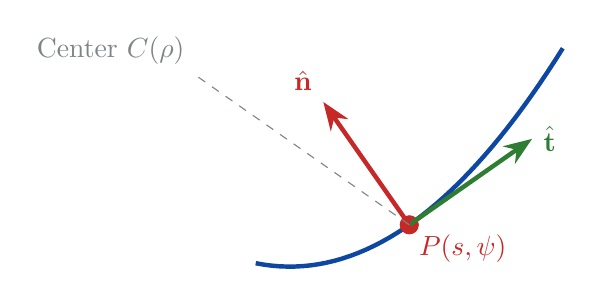
\begin{tikzpicture}[scale=1.3, >=Stealth]
    \draw[ultra thick, primaryblue, domain=0.5:3.5, samples=40] plot (\x, {0.3*\x*\x - 0.5*\x + 0.8});
    \coordinate (P) at (2.0, 1.0);
    \filldraw[accentred] (P) circle (2.5pt) node[below right] {$P(s, \psi)$};

    \draw[ultra thick, ->, accentgreen] (P) -- ($(P) + (1.2, 0.84)$) node[right] {$\hat{\mathbf{t}}$};
    \draw[ultra thick, ->, accentred] (P) -- ($(P) + (-0.84, 1.2)$) node[above left] {$\hat{\mathbf{n}}$};
    \draw[dashed, darkslate!60] (P) -- (-0.1, 2.47) node[above left] {Center $C(\rho)$};
\end{tikzpicture}
\end{center}

Velocity vector $\mathbf{v} = v \hat{\mathbf{t}} = \dot{s} \hat{\mathbf{t}}$. Acceleration $\mathbf{a} = \frac{d}{dt}(v \hat{\mathbf{t}}) = \dot{v} \hat{\mathbf{t}} + v \frac{d\hat{\mathbf{t}}}{dt}$.\\
Using chain rule $\frac{d\hat{\mathbf{t}}}{dt} = \frac{d\hat{\mathbf{t}}}{d\psi} \frac{d\psi}{ds} \frac{ds}{dt} = (\hat{\mathbf{n}}) \left(\frac{1}{\rho}\right) (v) = \frac{v}{\rho} \hat{\mathbf{n}}$:
\[
\mathbf{a} = \dot{v} \hat{\mathbf{t}} + \frac{v^2}{\rho} \hat{\mathbf{n}} \implies a_t = \dot{v} = v\frac{dv}{ds} = \ddot{s}, \quad a_n = \frac{v^2}{\rho}
\]
\end{proofbox}

\section{Angular Momentum \& Rectilinear SHM}

\begin{theorembox}{Proof 20: Conservation of Angular Momentum under Central Force}
For central force $\mathbf{F} = F(r)\hat{r}$, angular momentum per unit mass $h = r^2\dot{\theta}$ is constant.
\end{theorembox}

\begin{proofbox}{Derivation of Angular Momentum Conservation}
Transverse equation of motion under purely radial central force ($F_\theta = 0$):
\[
a_\theta = \frac{1}{r} \frac{d}{dt}(r^2 \dot{\theta}) = 0 \implies \frac{d}{dt}(r^2 \dot{\theta}) = 0 \implies r^2 \dot{\theta} = h = \text{constant}
\]
Areal velocity $\frac{dA}{dt} = \frac{1}{2} r^2 \dot{\theta} = \frac{h}{2} = \text{constant}$. Angular momentum $L = m r^2 \dot{\theta} = m h$ is strictly conserved.
\end{proofbox}

\begin{theorembox}{Proof 21, 22 \& 23: Velocity, Displacement, and Period in Rectilinear SHM}
For equation $\ddot{x} = -\mu x$:
1. \textbf{Velocity}: $v^2 = \mu(a^2 - x^2)$.
2. \textbf{Displacement}: $x(t) = a\cos(\sqrt{\mu}t)$ or $x(t) = a\sin(\sqrt{\mu}t)$.
3. \textbf{Period \& Frequency}: $T = \frac{2\pi}{\sqrt{\mu}}, n = \frac{\sqrt{\mu}}{2\pi}$.
\end{theorembox}

\begin{proofbox}{Derivation of SHM Formulae}
\begin{center}
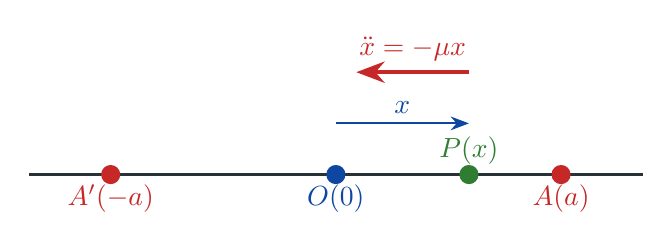
\begin{tikzpicture}[scale=1.3, >=Stealth]
    \draw[thick, darkslate] (-3.0, 0) -- (3.0, 0);
    \filldraw[accentred] (-2.2, 0) circle (2.5pt) node[below] {$A'(-a)$};
    \filldraw[primaryblue] (0, 0) circle (2.5pt) node[below] {$O(0)$};
    \filldraw[accentred] (2.2, 0) circle (2.5pt) node[below] {$A(a)$};
    \filldraw[accentgreen] (1.3, 0) circle (2.5pt) node[above] {$P(x)$};

    \draw[->, thick, primaryblue] (0, 0.5) -- (1.3, 0.5) node[midway, above] {$x$};
    \draw[->, ultra thick, accentred] (1.3, 1.0) -- (0.2, 1.0) node[midway, above] {$\ddot{x} = -\mu x$};
\end{tikzpicture}
\end{center}

Integrating $v \frac{dv}{dx} = -\mu x \implies \frac{v^2}{2} = -\mu \frac{x^2}{2} + C$. Using boundary condition $v = 0$ at $x = a \implies C = \frac{\mu a^2}{2} \implies v^2 = \mu(a^2 - x^2)$.\\
Integrating $\frac{dx}{\sqrt{a^2 - x^2}} = -\sqrt{\mu} dt \implies \cos^{-1}(x/a) = \sqrt{\mu} t \implies x(t) = a\cos(\sqrt{\mu}t)$.\\
Time taken for one full cycle $A \to A' \to A$: $\Delta(\sqrt{\mu}t) = 2\pi \implies T = \frac{2\pi}{\sqrt{\mu}}$, $n = 1/T = \frac{\sqrt{\mu}}{2\pi}$.
\end{proofbox}

% ==============================================================================
% UNIT IV: CENTRAL ORBITS, KEPLER'S LAWS & CONSTRAINED MOTION
% ==============================================================================
\chapter{Central Orbits, Kepler's Laws \& Constrained Motion}

\section{Differential Equations of Central Orbits}

\begin{theorembox}{Proof 24 \& 25: Polar and Pedal Equations of Central Orbits}
1. \textbf{Polar Form ($u=1/r$)}: $\frac{d^2u}{d\theta^2} + u = \frac{F(u)}{h^2 u^2}$.
2. \textbf{Pedal Form ($p=r\sin\phi$)}: $\frac{h^2}{p^3} \frac{dp}{dr} = F(r)$.
\end{theorembox}

\begin{proofbox}{Derivation of Polar and Pedal Orbit Equations}
\begin{center}
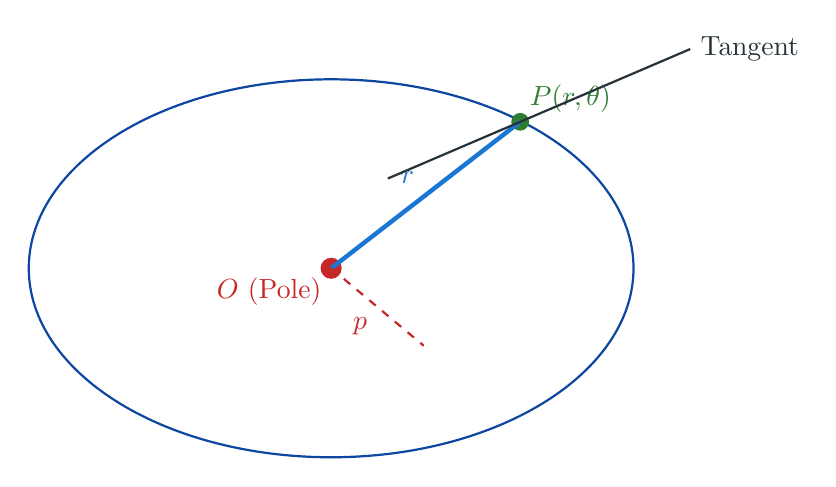
\begin{tikzpicture}[scale=1.2, >=Stealth]
    \filldraw[accentred] (0,0) circle (3pt) node[below left] {$O$ (Pole)};
    \draw[thick, primaryblue] (0,0) ellipse (3.2cm and 2.0cm);
    \coordinate (P) at (2.0, 1.55);
    \filldraw[accentgreen] (P) circle (2.5pt) node[above right] {$P(r, \theta)$};
    \draw[ultra thick, secondaryblue] (0,0) -- (P) node[midway, above left] {$r$};
    \draw[thick, darkslate] ($(P) + (-1.4, -0.6)$) -- ($(P) + (1.8, 0.77)$) node[right] {Tangent};
    \draw[dashed, accentred, thick] (0,0) -- (0.98, -0.82) node[midway, below left] {$p$};
\end{tikzpicture}
\end{center}

Radial equation: $\ddot{r} - r\dot{\theta}^2 = -F$. Substituting $r = 1/u$ and $\dot{\theta} = h u^2$:
\[
\dot{r} = \frac{d}{d\theta}\left(\frac{1}{u}\right) \dot{\theta} = -\frac{1}{u^2}\frac{du}{d\theta}(h u^2) = -h \frac{du}{d\theta} \implies \ddot{r} = -h \frac{d^2u}{d\theta^2} \dot{\theta} = -h^2 u^2 \frac{d^2u}{d\theta^2}
\]
Substituting into radial equation: $-h^2 u^2 \frac{d^2u}{d\theta^2} - \frac{1}{u}(h^2 u^4) = -F \implies \frac{d^2u}{d\theta^2} + u = \frac{F}{h^2 u^2}$.\\
For pedal form, $1/p^2 = u^2 + (du/d\theta)^2$. Differentiating wrt $\theta$: $-\frac{2}{p^3}\frac{dp}{d\theta} = 2u\frac{du}{d\theta} + 2\frac{du}{d\theta}\frac{d^2u}{d\theta^2} = 2\frac{du}{d\theta}\left(u + \frac{d^2u}{d\theta^2}\right) = 2\frac{du}{d\theta}\frac{F}{h^2 u^2}$.
Since $\frac{dp}{d\theta} = \frac{dp}{dr}\frac{dr}{d\theta} = \frac{dp}{dr}\left(-\frac{1}{u^2}\frac{du}{d\theta}\right)$, simplifying yields $\frac{h^2}{p^3}\frac{dp}{dr} = F(r)$.
\end{proofbox}

\begin{theorembox}{Proof 26: Velocity at Any Point of Central Orbit}
\begin{equation}
v^2 = h^2 \left[ u^2 + \left(\frac{du}{d\theta}\right)^2 \right] = \frac{h^2}{p^2}
\end{equation}
\end{theorembox}

\begin{proofbox}{Derivation of Orbit Velocity Formula}
Radial velocity $v_r = \dot{r} = -h \frac{du}{d\theta}$, transverse velocity $v_\theta = r\dot{\theta} = h u$.\\
Total speed squared: $v^2 = v_r^2 + v_\theta^2 = h^2 \left[ u^2 + \left(\frac{du}{d\theta}\right)^2 \right]$.\\
Using pedal relation $p = r\sin\phi \implies v = \frac{r\dot{\theta}}{\sin\phi} = \frac{h}{p} \implies v^2 = \frac{h^2}{p^2}$.
\end{proofbox}

\section{Inverse Square Law \& Kepler's Laws}

\begin{theorembox}{Proof 27, 28, 29 \& 30: Conic Orbits and Kepler's Three Laws}
Under central force $F = \mu/r^2$:
1. \textbf{First Law}: Orbit is conic $l/r = 1 + e\cos\theta$ ($l = h^2/\mu$). Ellipse for $e<1$ ($v^2 = \mu(2/r - 1/a)$).
2. \textbf{Second Law}: Areal velocity is constant ($\frac{dA}{dt} = \frac{h}{2}$).
3. \textbf{Third Law}: Period squared $T^2 = \frac{4\pi^2}{\mu} a^3 \implies T^2 \propto a^3$.
\end{theorembox}

\begin{proofbox}{Derivation of Inverse Square Law \& Kepler's Laws}
\begin{center}
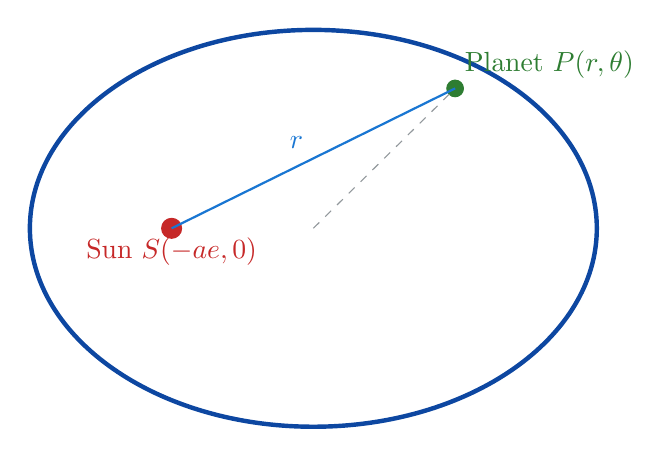
\begin{tikzpicture}[scale=1.2, >=Stealth]
    \filldraw[accentred] (-1.5,0) circle (3pt) node[below] {Sun $S(-ae, 0)$};
    \draw[ultra thick, primaryblue] (0,0) ellipse (3.0cm and 2.1cm);
    \coordinate (P) at (1.5, 1.48);
    \filldraw[accentgreen] (P) circle (2.5pt) node[above right] {Planet $P(r,\theta)$};
    \draw[thick, secondaryblue] (-1.5,0) -- (P) node[midway, above left] {$r$};
    \draw[dashed, darkslate!50] (0,0) -- (P);
\end{tikzpicture}
\end{center}

For $F = \mu u^2$, polar equation becomes $\frac{d^2u}{d\theta^2} + u = \frac{\mu}{h^2}$. General solution $u = \frac{\mu}{h^2}[1 + e\cos(\theta - \theta_0)] \implies \frac{l}{r} = 1 + e\cos\theta$ where $l = h^2/\mu$. This proves Kepler's 1st Law (Elliptic orbit with Sun at focus for $e<1$).\\
Kepler's 2nd Law follows directly from transverse equation $r^2\dot{\theta} = h \implies \frac{dA}{dt} = \frac{h}{2} = \text{const}$.\\
For Kepler's 3rd Law, total area of ellipse is $\pi a b$. Period $T = \frac{\text{Total Area}}{\text{Areal Velocity}} = \frac{\pi a b}{h/2} = \frac{2\pi a b}{h}$.
Since $b^2 = a l = a(h^2/\mu) \implies h = \sqrt{\mu l} = \frac{b\sqrt{\mu}}{\sqrt{a}}$:
\[
T = \frac{2\pi a b}{b\sqrt{\mu}/\sqrt{a}} = \frac{2\pi a^{3/2}}{\sqrt{\mu}} \implies T^2 = \left(\frac{4\pi^2}{\mu}\right) a^3 \implies T^2 \propto a^3
\]
\end{proofbox}

\section{Constrained Motion on Vertical Curves}

\begin{theorembox}{Proof 31 \& 32: Motion on Smooth Vertical Circle}
1. \textbf{Velocity \& Reaction}: $v^2 = u^2 - 2ga(1-\cos\theta), N = \frac{m}{a}[u^2 - 2ga + 3ga\cos\theta]$. Loop complete if $u \ge \sqrt{5ga}$.
2. \textbf{Small Oscillations}: $\ddot{s} \approx -\left(\frac{g}{a}\right)s \implies T = 2\pi\sqrt{\frac{a}{g}}$.
\end{theorembox}

\begin{proofbox}{Derivation of Vertical Circle Motion}
\begin{center}
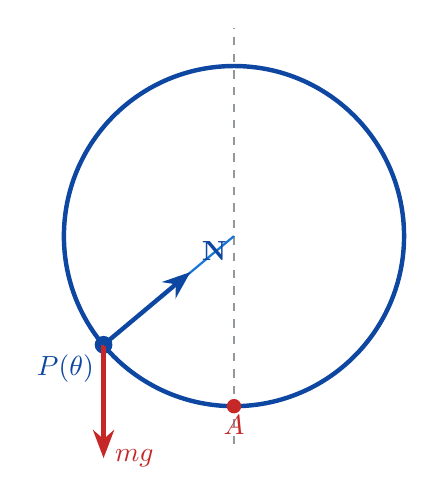
\begin{tikzpicture}[scale=1.2, >=Stealth]
    \coordinate (O) at (0,0);
    \draw[ultra thick, primaryblue] (O) circle (1.8);
    \draw[dashed, darkslate!50] (0, -2.2) -- (0, 2.2);
    \filldraw[accentred] (0,-1.8) circle (2pt) node[below] {$A$};
    \coordinate (P) at (-1.38, -1.15);
    \filldraw[primaryblue] (P) circle (2.5pt) node[below left] {$P(\theta)$};
    \draw[thick, secondaryblue] (O) -- (P);
    \draw[ultra thick, ->, accentred] (P) -- ++(0, -1.2) node[right] {$mg$};
    \draw[ultra thick, ->, primaryblue] (P) -- ++(0.92, 0.77) node[above right] {$\mathbf{N}$};
\end{tikzpicture}
\end{center}

Tangential equation $m v \frac{dv}{ds} = -mg \sin\theta$. With $s = a\theta$, $v \frac{dv}{d\theta} = -ga \sin\theta$. Integrating from $\theta=0 (v=u)$: $v^2 = u^2 - 2ga(1 - \cos\theta)$.\\
Normal equation $\frac{m v^2}{a} = N - mg \cos\theta \implies N = mg\cos\theta + \frac{m}{a}[u^2 - 2ga(1-\cos\theta)] = \frac{m}{a}[u^2 - 2ga + 3ga\cos\theta]$.\\
For small $\theta$, $\sin\theta \approx \theta = s/a \implies \ddot{s} = -g(s/a) \implies T = 2\pi\sqrt{a/g}$.
\end{proofbox}

\begin{theorembox}{Proof 33 \& 34: Motion on Vertical Cycloid (Isochronous SHM)}
For cycloid $s = 4a\sin\psi$: $\ddot{s} = -g\sin\psi = -\left(\frac{g}{4a}\right)s$.
Exact isochronous SHM with $T = 4\pi\sqrt{\frac{a}{g}}$ and fall time to vertex $t_{\text{vertex}} = \pi\sqrt{\frac{a}{g}}$.
\end{theorembox}

\begin{proofbox}{Derivation of Cycloidal SHM}
\begin{center}
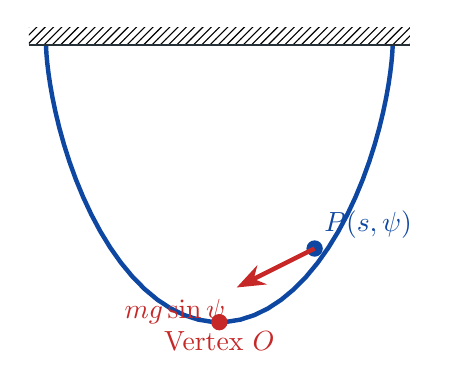
\begin{tikzpicture}[scale=1.1, >=Stealth]
    \draw[ultra thick, primaryblue, domain=-1.57:1.57, samples=50] plot ({2*(2*\x + sin(2*\x r))/3.14}, {1.6*(1 - cos(2*\x r))});
    \fill[pattern=north east lines] (-2.2, 3.2) rectangle (2.2, 3.4);
    \draw[thick, darkslate] (-2.2, 3.2) -- (2.2, 3.2);
    \filldraw[accentred] (0,0) circle (2.5pt) node[below] {Vertex $O$};
    \coordinate (P) at (1.1, 0.85);
    \filldraw[primaryblue] (P) circle (2.5pt) node[above right] {$P(s,\psi)$};
    \draw[ultra thick, ->, accentred] (P) -- ++(-0.9, -0.45) node[below left] {$mg\sin\psi$};
\end{tikzpicture}
\end{center}

Equation of motion along cycloid arc $s$: $\ddot{s} = -g\sin\psi$. Substituting intrinsic cycloid formula $\sin\psi = s/(4a)$:
\[
\ddot{s} = -\left(\frac{g}{4a}\right) s \implies \text{Exact SHM } \ddot{s} = -\omega^2 s \quad \text{where } \omega = \sqrt{\frac{g}{4a}} = \frac{1}{2}\sqrt{\frac{g}{a}}
\]
Time period $T = \frac{2\pi}{\omega} = \frac{2\pi}{\frac{1}{2}\sqrt{g/a}} = 4\pi\sqrt{\frac{a}{g}}$ (Isochronous, independent of amplitude $s_0$).\\
Integrating $\dot{s}^2 = \omega^2(s_0^2 - s^2) \implies t = \frac{1}{\omega}\cos^{-1}(s/s_0) = 2\sqrt{\frac{a}{g}}\cos^{-1}\left(\frac{\sin\psi}{\sin\psi_0}\right)$. Fall to vertex ($s=0$) takes $t_{\text{vertex}} = \frac{\pi}{2\omega} = \pi\sqrt{\frac{a}{g}}$.
\end{proofbox}

% ==============================================================================
% UNIT V: FORCES IN 3D, DYNAME, POINSOT'S CENTRAL AXIS & MOMENTS OF INERTIA
% ==============================================================================
\chapter{Forces in 3D, Dyname, Poinsot's Central Axis \& Moments of Inertia}

\section{Reduction of 3D Forces \& Poinsot's Central Axis}

\begin{theorembox}{Proof 35, 36 \& 37: 3D Force Reduction, Pitch, and Poinsot's Central Axis}
1. \textbf{Reduction}: 3D forces reduce at $O$ to force $\mathbf{R}(X,Y,Z)$ and couple $\mathbf{G}(L,M,N)$.
2. \textbf{Pitch}: $p = \frac{\mathbf{R} \cdot \mathbf{G}}{R^2} = \frac{XL + YM + ZN}{X^2 + Y^2 + Z^2}$.
3. \textbf{Central Axis}: Equation of Poinsot's Central Axis:
\begin{equation}
\frac{L - (yZ - zY)}{X} = \frac{M - (zX - xZ)}{Y} = \frac{N - (xY - yX)}{Z} = p
\end{equation}
\end{theorembox}

\begin{proofbox}{Derivation of Poinsot's Central Axis}
\begin{center}
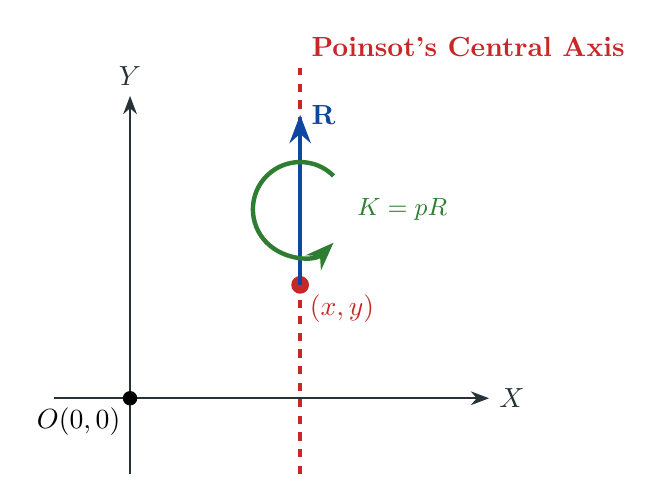
\begin{tikzpicture}[scale=1.2, >=Stealth]
    \draw[ultra thick, dashed, accentred] (1.8, -0.8) -- (1.8, 3.5) node[above right, font=\bfseries] {Poinsot's Central Axis};
    \draw[->, thick, darkslate] (-0.8, 0) -- (3.8, 0) node[right] {$X$};
    \draw[->, thick, darkslate] (0, -0.8) -- (0, 3.2) node[above] {$Y$};
    \filldraw[black] (0,0) circle (2pt) node[below left] {$O(0,0)$};
    \filldraw[accentred] (1.8, 1.2) circle (2.5pt) node[below right] {$(x, y)$};
    \draw[ultra thick, ->, primaryblue] (1.8, 1.2) -- (1.8, 3.0) node[right] {$\mathbf{R}$};
    \draw[ultra thick, ->, accentgreen] (1.8, 2.0) ++(45:0.5) arc (45:315:0.5);
    \node[accentgreen, font=\small, right] at (2.3, 2.0) {$K = p R$};
\end{tikzpicture}
\end{center}

Forces $\mathbf{F}_i(X_i, Y_i, Z_i)$ at $(x_i, y_i, z_i)$ reduce at origin $O$ to $\mathbf{R} = (\sum X_i, \sum Y_i, \sum Z_i)$ and couple $\mathbf{G} = (L, M, N)$ where $L = \sum(y_i Z_i - z_i Y_i), M = \sum(z_i X_i - x_i Z_i), N = \sum(x_i Y_i - y_i X_i)$.\\
Shifting origin to $O'(x, y, z)$, new couple components are $L' = L - (yZ - zY), M' = M - (zX - xZ), N' = N - (xY - yX)$.\\
For $O'(x,y,z)$ to lie on Central Axis, couple vector $\mathbf{G}'$ must be parallel to force $\mathbf{R}$ ($\mathbf{G}' = p \mathbf{R}$):
\[
\frac{L'}{X} = \frac{M'}{Y} = \frac{N'}{Z} = p \implies \frac{L - (yZ - zY)}{X} = \frac{M - (zX - xZ)}{Y} = \frac{N - (xY - yX)}{Z} = p
\]
\end{proofbox}

\section{Moments of Inertia Theorems \& Standard Bodies}

\begin{theorembox}{Proof 38 \& 39: Parallel and Perpendicular Axes Theorems}
1. \textbf{Parallel Axes Theorem}: $I_{L'} = I_{\text{cm}} + M d^2$.
2. \textbf{Perpendicular Axes Theorem (Plane Lamina)}: $I_z = I_x + I_y$.
\end{theorembox}

\begin{proofbox}{Derivation of M.I. Theorems}
\begin{center}
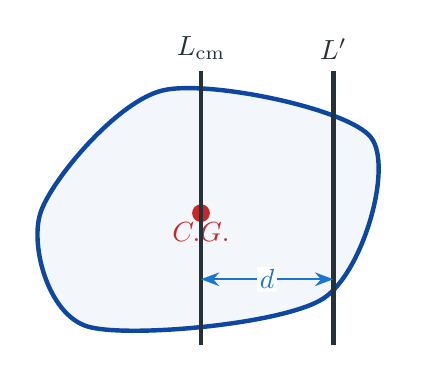
\begin{tikzpicture}[scale=1.2, >=Stealth]
    \draw[ultra thick, primaryblue, fill=primaryblue!5] plot [smooth cycle] coordinates {(0,0) (2.5,0.3) (3.0,2.0) (0.8,2.5) (-0.5,1.2)};
    \filldraw[accentred] (1.2, 1.2) circle (2.5pt) node[below] {$C.G.$};
    \draw[ultra thick, darkslate] (1.2, -0.2) -- (1.2, 2.7) node[above] {$L_{\text{cm}}$};
    \draw[ultra thick, darkslate] (2.6, -0.2) -- (2.6, 2.7) node[above] {$L'$};
    \draw[thick, <->, secondaryblue] (1.2, 0.5) -- (2.6, 0.5) node[midway, fill=white, inner sep=1pt] {$d$};
\end{tikzpicture}
\end{center}

For Parallel Axes Theorem, let mass element $m_i$ be at distance $r_i$ from C.G. axis $L_{\text{cm}}$. Distance from parallel axis $L'$ is $r'_i = r_i + d$:
\[
I_{L'} = \sum m_i (r_i + d)^2 = \sum m_i r_i^2 + 2d \sum m_i r_i + d^2 \sum m_i = I_{\text{cm}} + 0 + M d^2 = I_{\text{cm}} + M d^2
\]
For Perpendicular Axes Theorem of plane lamina in $XY$ plane ($z_i = 0$):
\[
I_x + I_y = \sum m_i y_i^2 + \sum m_i x_i^2 = \sum m_i (x_i^2 + y_i^2) = I_z
\]
\end{proofbox}

\begin{theorembox}{Proof 40: Standard Moments of Inertia Derivations}
Integrations for symmetric bodies: Thin Rod ($I = \frac{1}{3}ma^2$), Circular Disc ($I = \frac{1}{2}ma^2$), Solid Sphere ($I = \frac{2}{5}ma^2$).
\end{theorembox}

\begin{proofbox}{Derivation of Standard M.I. Formulae}
\begin{center}
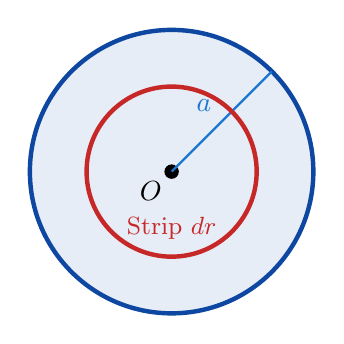
\begin{tikzpicture}[scale=1.2, >=Stealth]
    \draw[ultra thick, primaryblue, fill=primaryblue!10] (0,0) circle (1.5);
    \filldraw[black] (0,0) circle (2pt) node[below left] {$O$};
    \draw[thick, secondaryblue] (0,0) -- (1.06, 1.06) node[midway, above left] {$a$};
    \draw[ultra thick, accentred] (0,0) circle (0.9);
    \node[accentred, font=\small] at (0, -0.6) {Strip $dr$};
\end{tikzpicture}
\end{center}

For a circular disc of mass $m$ and radius $a$, surface density $\sigma = \frac{m}{\pi a^2}$. Consider a thin concentric ring of radius $r$ and width $dr$. Mass of ring $dm = \sigma (2\pi r dr) = \frac{2m}{a^2} r dr$.\\
Moment of inertia of ring about central axis $dI = dm \cdot r^2 = \frac{2m}{a^2} r^3 dr$. Integrating from $r=0$ to $r=a$:
\[
I_{\text{axis}} = \int_0^a \frac{2m}{a^2} r^3 dr = \frac{2m}{a^2} \left[ \frac{r^4}{4} \right]_0^a = \frac{1}{2} m a^2
\]
Using Perpendicular Axes Theorem $I_z = I_x + I_y = 2 I_{\text{dia}} \implies I_{\text{dia}} = \frac{1}{2} I_{\text{axis}} = \frac{1}{4} m a^2$.
\end{proofbox}

\section{Inclined Lines \& Momental Ellipsoid}

\begin{theorembox}{Proof 41 \& 42: M.I. About Inclined Line \& Momental Ellipsoid}
1. \textbf{Inclined Line $(\alpha, \beta, \gamma)$}: $I = I_{xx}\alpha^2 + I_{yy}\beta^2 + I_{zz}\gamma^2 - 2I_{xy}\alpha\beta - 2I_{yz}\beta\gamma - 2I_{zx}\gamma\alpha$.
2. \textbf{Momental Ellipsoid}: Quadric surface $I_{xx}x^2 + I_{yy}y^2 + I_{zz}z^2 - 2I_{xy}xy - 2I_{yz}yz - 2I_{zx}zx = 1$.
\end{theorembox}

\begin{proofbox}{Derivation of Inclined Line M.I. and Momental Ellipsoid}
\begin{center}
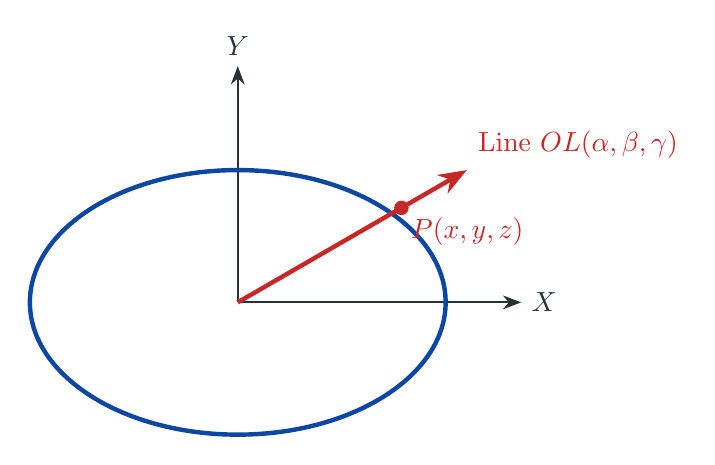
\begin{tikzpicture}[scale=1.2, >=Stealth]
    \draw[->, thick, darkslate] (0,0) -- (3.0,0) node[right] {$X$};
    \draw[->, thick, darkslate] (0,0) -- (0,2.5) node[above] {$Y$};
    \draw[ultra thick, primaryblue] (0,0) ellipse (2.2cm and 1.4cm);
    \draw[ultra thick, ->, accentred] (0,0) -- (30:2.8) node[above right] {Line $OL(\alpha,\beta,\gamma)$};
    \filldraw[accentred] (30:2.0) circle (2pt) node[below right] {$P(x,y,z)$};
\end{tikzpicture}
\end{center}

Perpendicular distance $p_i$ of mass $m_i(x_i, y_i, z_i)$ from line $OL(\alpha,\beta,\gamma)$ satisfies $p_i^2 = (x_i^2+y_i^2+z_i^2)(\alpha^2+\beta^2+\gamma^2) - (\alpha x_i + \beta y_i + \gamma z_i)^2$. Summing over $m_i$:
\[
I_{OL} = I_{xx}\alpha^2 + I_{yy}\beta^2 + I_{zz}\gamma^2 - 2I_{xy}\alpha\beta - 2I_{yz}\beta\gamma - 2I_{zx}\gamma\alpha
\]
Set point $P(x,y,z)$ on line $OL$ at distance $r = 1/\sqrt{I_{OL}}$ from origin $O$. Then $x = r\alpha, y = r\beta, z = r\gamma \implies \alpha = x/r, \beta = y/r, \gamma = z/r$. Substituting into $I_{OL}$:
\[
I_{OL} = I_{xx}\left(\frac{x}{r}\right)^2 + I_{yy}\left(\frac{y}{r}\right)^2 + I_{zz}\left(\frac{z}{r}\right)^2 - 2I_{xy}\frac{xy}{r^2} - 2I_{yz}\frac{yz}{r^2} - 2I_{zx}\frac{zx}{r^2}
\]
Multiplying by $r^2 = 1/I_{OL}$ yields the equation of the **Momental Ellipsoid**:
\[
I_{xx}x^2 + I_{yy}y^2 + I_{zz}z^2 - 2I_{xy}xy - 2I_{yz}yz - 2I_{zx}zx = 1
\]
\end{proofbox}

\end{document}
